% Preamble
\documentclass[../Relazione_circuiti]{subfiles}
% \usepackage{amstex} Mi si era aggiunto da solo, magari un giorno capiamo che serve

% Packages
\graphicspath{{\subfix{../images/}}}

% Document
\begin{document}

Questo esperimento vuole verificare la validità delle formule teoriche su un filtro crossover reale. \\ \\
Il filtro crossover è un circuito RLC costituito da due rami: uno con un filtro passa basso realizzato mediante un
induttore (ramo \textbf{Woofer}), l'altro con un filtro passa alto costituito da un condensatore (ramo
\textbf{Tweeter}).

\begin{figure}[H]
  \centering
  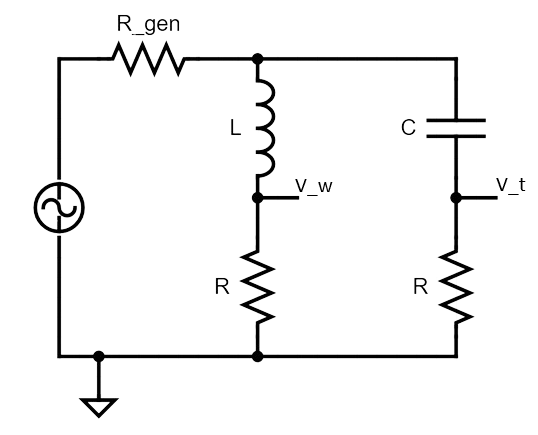
\includegraphics[width=8cm]{Schema_crossover.png}

  \caption{Schema del circuito realizzato}
  \label{fig:schema_circuito}

\end{figure}

Le due resistenze nella Fig. \ref{fig:schema_circuito} simulano degli altoparlanti (da qui i nomi dei rami), e sono da
considerarsi uguali a meno delle incertezze.

Le componenti di un segnale oscillante in ingresso, vengono scalate in ampiezza sui rami del circuito in base alla loro
frequenza.
Il ramo del \textit{woofer} presenta un'attenuazione progressiva delle componenti ad alta frequenza, mentre il ramo
del \textit{tweeter} di quelle a bassa.\\
La frequenza alla quale un segnale è ripartito in egual modo sui due rami è detta \textit{frequenza di cross} e dipende
dai valori della capacità e dell'induttanza del circuito.
Per calcolarla basta eguagliare le impedenze dei due rami, e si ottiene facilmente:

\begin{equation}
  \label{eq:f_cross}
  f_{cross} = \frac{1}{2 \pi \sqrt{LC} }
\end{equation}

dove $L$ è l'induttanza della bobina sul ramo Woofer e $C$ la capacità del condensatore sul ramo Tweeter.

Sempre alla frequenza di cross, si ha anche uno sfasamento dei due rami rispetto al generatore uguale e opposto: il
Woofer anticipa, il Tweeter ritarda.

\begin{align}
  \phi_{woofer} &= \arctan(-\frac{\omega L}{R}) \label{eq:p_woofer} \\
  \phi_{tweeter} &= \arctan(\frac{1}{\omega RC}) \label{eq:p_tweeter}
\end{align}

dove $L$ e $C$ sono definiti come nell'Eq. \eqref{eq:f_cross}, $\omega$ è la pulsazione dell'onda in ingresso e $R$ il
valore delle resistenze sui due rami.


\end{document}